\documentclass{article}
\usepackage{geometry}
 \geometry{
 a4paper,
 total={170mm,270mm},
 left=20mm,
 top=10mm,
 }
\usepackage{graphicx}
\usepackage{listings}
\usepackage{float}
\usepackage{enumitem}
\usepackage{caption}
\usepackage{amsmath}
\usepackage{datetime}
\usepackage{multirow}
\newcommand*{\addheight}[2][.5ex]{%
  \raisebox{0pt}[\dimexpr\height+(#1)\relax]{#2}%
}
\newdate{date}{14}{10}{2016}
\date{\displaydate{date}}
\title{\textbf{Machine Learning - CSCI 5622} \\
HW 5 - Learnability}
\author{\textbf{Santhanakrishnan Ramani}}
\begin{document}
\maketitle

\section*{Problem 1}
To find a bound on the number of randomly drawn training examples sufficient to assure that for any target class c in given C, any consistent learner using H=C will, with probability 95\%, output a hypothesis with error at most 0.15.\\

The number of possible hypothesis is the number of triangles that can be formed. Since the number of triangles that can be formed is $\binom{N}{3}$ where N is the number of points in the grid which is equal to 10000 in this case.\\

The number of triangles = No of Hypothesis (H) $ = \dfrac{10000 * 9999 * 9998}{6} = 166616670000$.\\

Given,  $\epsilon = 0.15$ and  $\delta = 0.05$\\

The bound on the number of samples with finite consistent hypothesis class can be found using the formula,
$$m \geq \dfrac{1}{\epsilon}(ln|H| + ln \dfrac{1}{\delta})$$

Substituting all the values in the above formula we get, $m \geq 192.23$\\

Therefore, we need a minimum of 193 samples for the given condition.

\section*{Problem 2}
To state and prove the VC Dimension of the hypothesis class H of linear hyperplanes in 2D that passes through the origin.

\begin{table}[H]
\centering
\begin{tabular}{|c|c|}
	\hline
	\addheight{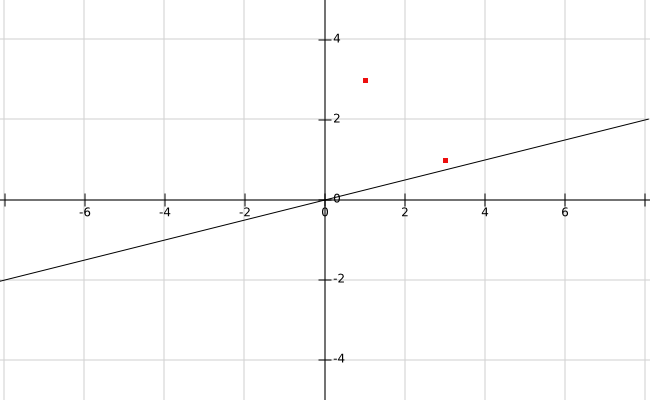
\includegraphics[width=70mm]{images/0.png}} &
	\addheight{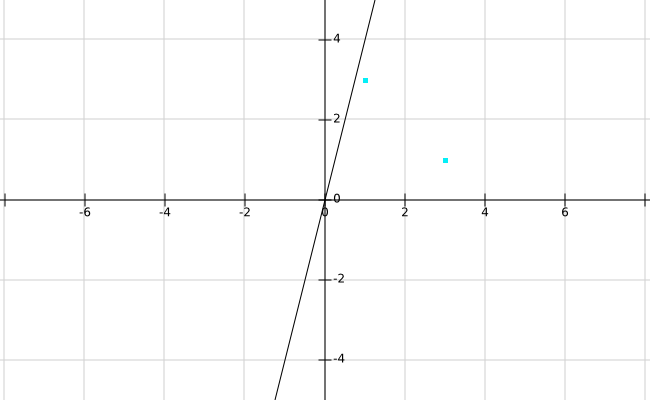
\includegraphics[width=70mm]{images/3.png}} \\
	\hline
	\addheight{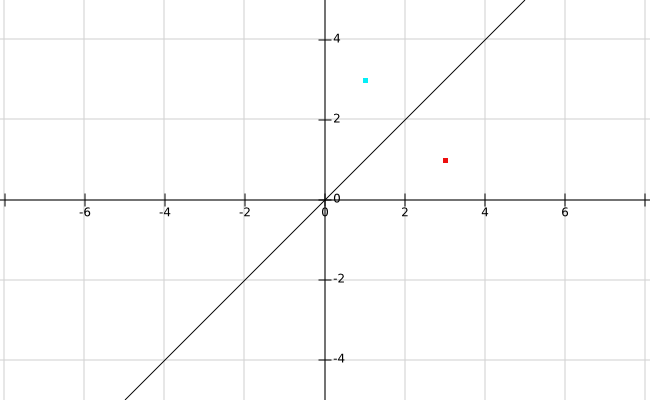
\includegraphics[width=70mm]{images/1.png}} &
	\addheight{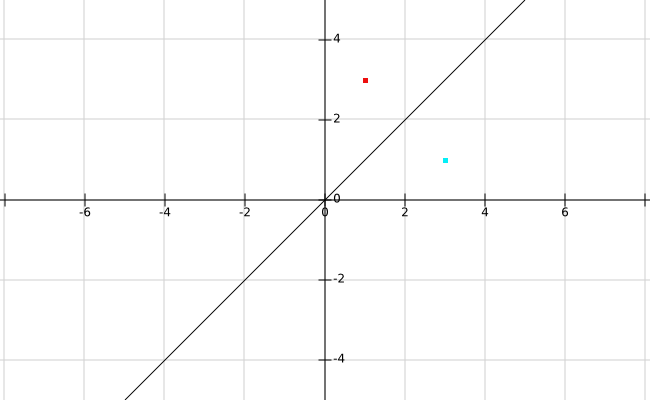
\includegraphics[width=70mm]{images/2.png}} \\
	\hline
\end{tabular}
\end{table}

The figures above shows us an example of a configuration of 2 points that can be shattered by H. Therefore, we can conclude that the lower bound on the VC Dimension is 2.

In order to prove that upper bound on the VC Dimension, lets assume that there exists a set S, s.t $|S| = 3$ that can be shattered by H. Let us assume $(x_1,y_1) (x_2,y_2) (x_3,y_3)$ be some arbitrary three points s.t. $x_1 \leq x_2 \leq x_3$ and $y_1 \geq y_2 \geq y_3$ and let their respective labellings be $l=(-1, +1, -1)$ and there exists some $h = wx$ (equation of a hyperplane and assuming w is positive as there can't be a hyperplane with negative slope passing through the origin in the first quadrant) that works.\\

Since,
\begin{equation}
l_1 = -1 \implies y_1 < wx
\end{equation}
\begin{equation}
l_2 = +1 \implies y_2 \geq wx
\end{equation}
\begin{equation}
l_3 = -1 \implies y_3 < wx 
\end{equation}

From Eq (1), (2) \& (3) we get,
$$y_1 \,\&\, y_3 \leq y_2 $$

Which contradicts our assumption $y_1 \geq y_2 \geq y_3 \implies$ that the $VCdim(H) < 3$.\\

Combining it with lower bound we can conclude that the $VCdim(H) = 2$
\section*{Problem 3}

In order to find the W value that shatters all the points, I ran a loop of different W values and found the one that shatters a particular combination of training points. After trying it with different combinations, I was able to see the pattern in W and obtain a closed form expression for it. Found out that the W is one plus sum of all the data point raised to the power of 2 which are classified as negative in the training samples multiplied by $\pi$.Since, we were able to get a closed form expression for W, we can shatter any points of the form $2^{-k}$ using sine functions, which implies that it's VC Dimension is $\infty$.

\begin{table}[H]
\centering
\caption{Sample Combinations \& W value}
\label{my-label}
\begin{tabular}{|l|l|}
\hline
Training example  Combinations & W \\
\hline
kSIMPLE\_TRAIN = {[}(1, True), (2, True), (4, True), (5, True){]}   & 1  \\
kSIMPLE\_TRAIN = {[}(1, False), (2, True), (4, True), (5, True){]}  & 3  \\
kSIMPLE\_TRAIN = {[}(1, True), (2, False), (4, True), (5, True){]}  & 5  \\
kSIMPLE\_TRAIN = {[}(1, True), (2, True), (4, False), (5, True){]}  & 17 \\
kSIMPLE\_TRAIN = {[}(1, True), (2, True), (4, True), (5, False){]}  & 33 \\
kSIMPLE\_TRAIN = {[}(1, False), (2, False), (4, True), (5, True){]} & 7  \\
kSIMPLE\_TRAIN = {[}(1, False), (2, True), (4, False), (5, True){]} & 19 \\
kSIMPLE\_TRAIN = {[}(1, False), (2, True), (4, True), (5, False){]} & 35 \\
\hline
\end{tabular}
\end{table}

$$ w = [1 + \sum_{i=1}^{m} \dfrac{(1-y_i)}{2} 2^{x_i}] \pi$$  

This shows us that, only the negative examples contribute in the calculation of W.
Which seems pretty reasonable as smaller the values that gets labelled as negative, the frequency of the sine curve will be higher and vice versa.\\

In order to classify the points as positive and negative the $sign(sin(wx))$ is positive or negative respectively. So, the value of $wx$ must be in the range of $[0,\pi]$ to be classified as positive and $(\pi,2\pi)$ to be classified as negative. So, the W stated above plays a crucial part in placing the values in their respective range in order for them to be classified correctly.
\end{document}
	